% Original text commented below .. please fill the refs, some from commented text below 
% Include also Sarrof et al, Nunez-Molina et al ..

Recent work  has studied the  ability of transformers to learn world models from next-token prediction
\citep{Toshniwal_Wiseman_Livescu_Gimpel_2022,li_iclr,nanda2023linear,world-models2,vafa2025what}  and
to generalize in length \citep{kazemnejad2023impact,zhou2024algorithms,huang2025formal}. 
\citet{sarrof2026verify} have  addressed a related problem that involves
generalization in the number of objects as well, and which results 
from the verification of  plans in the lifted \strips setting, 
where difference domain instances share the same action schemas
and predicate symbols but not the same set of objects
\citep{russell:book}.  Finally,  \citet{nunez2026strips} have used transformers to learn propositional \strips models
from action sequences for use with  classical planners off-the-shelf \citep{ghallab:book,geffner:book}.

In this work, we bring these different threads together by addressing the problem of \emph{learning lifted \strips models} from suitable traces using  a transformer architecture.
The problem involves a particular class of deterministic world-models  where actions add and delete atoms from the state  provided that the
precondition atoms are true. The atoms represent Boolean variables, yet the number of atoms in a domain vary with the number of instances.
As a result, the training and testing traces not only vary in length but also in the number of objects involved.
  
We consider two learning settings and two different transformer archiectures. In the first learning setting, the input traces  from which the \strips model are learned encode
action sequences and an initial state. Some of these traces are positive, if the action sequences are applicable in the given initial state, or negative if they are not.
In this setting, a single state is observed, the initial state, and traces can be positive or negative. In the second learning setting, the traces are all positive,
and they are ``labeled''  with the resulting  final state. The first type of traces are  related to those used by \citep{nunez2026strips} to learn \emph{propositional \strips} models,
while the second type of traces are related to those used by \citet{sarrof2026verify}  to verify plans given the planning domain,  in the lifted \strips settings.
Note that while in the two learning settings, the predicates  of the "hidden" domain are assumed to be known, no \emph{state transition} is fully or partially
observed. 

\begin{figure*}[!t]
    \centering    
%    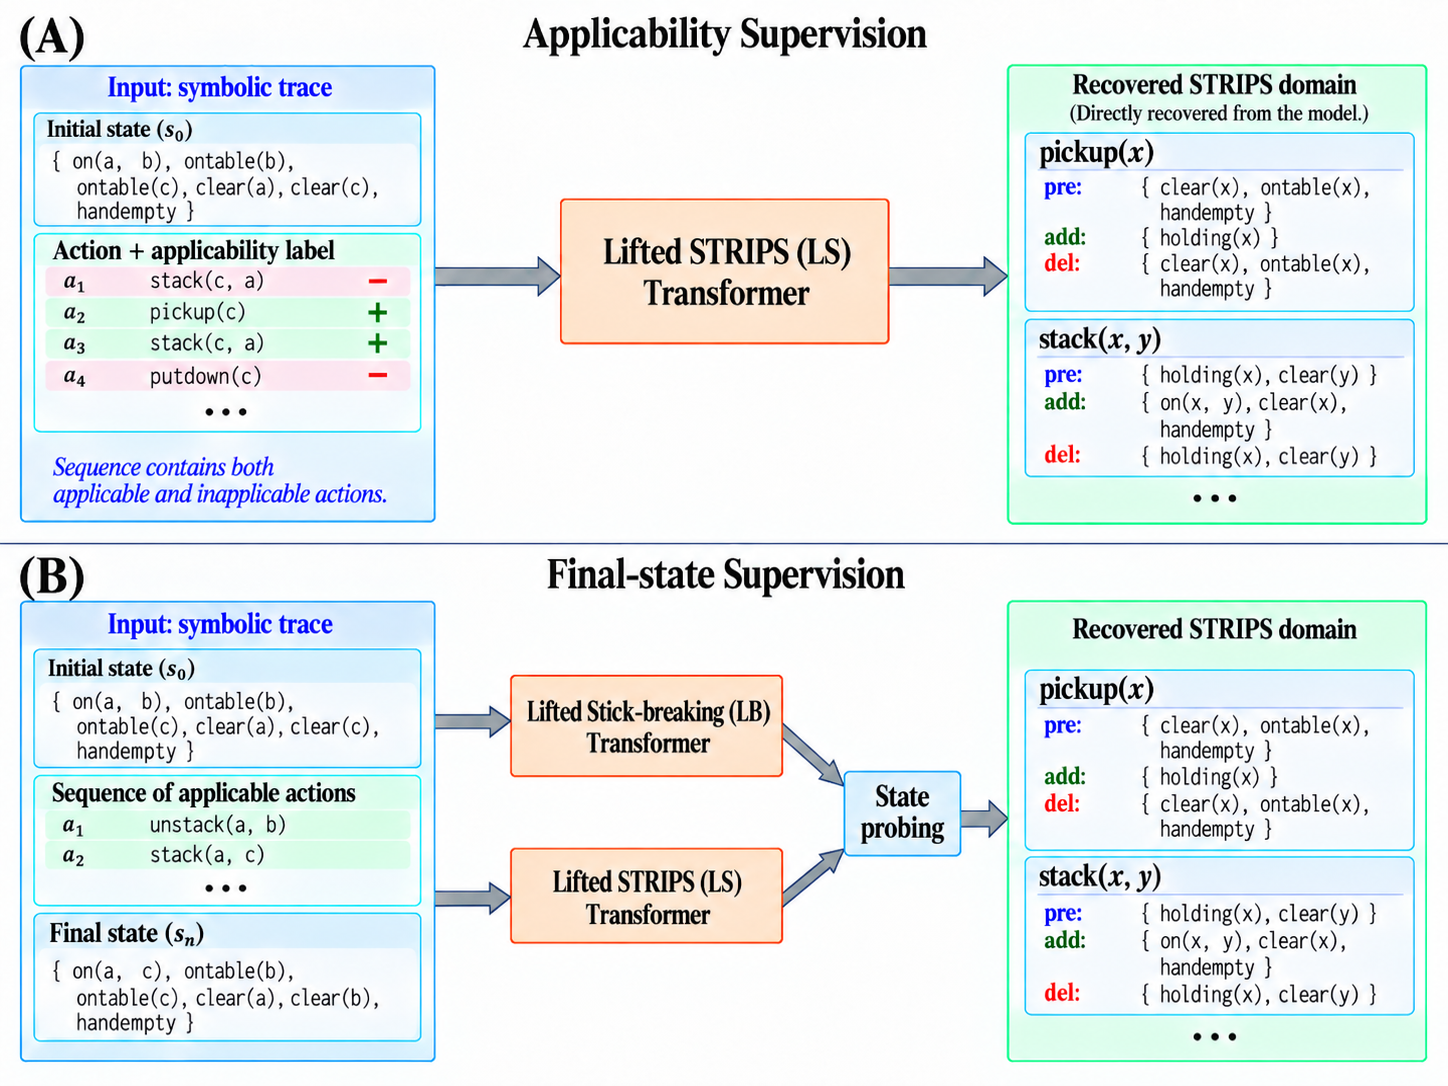
\includegraphics[width=\textwidth]{combined2_A.png}
%    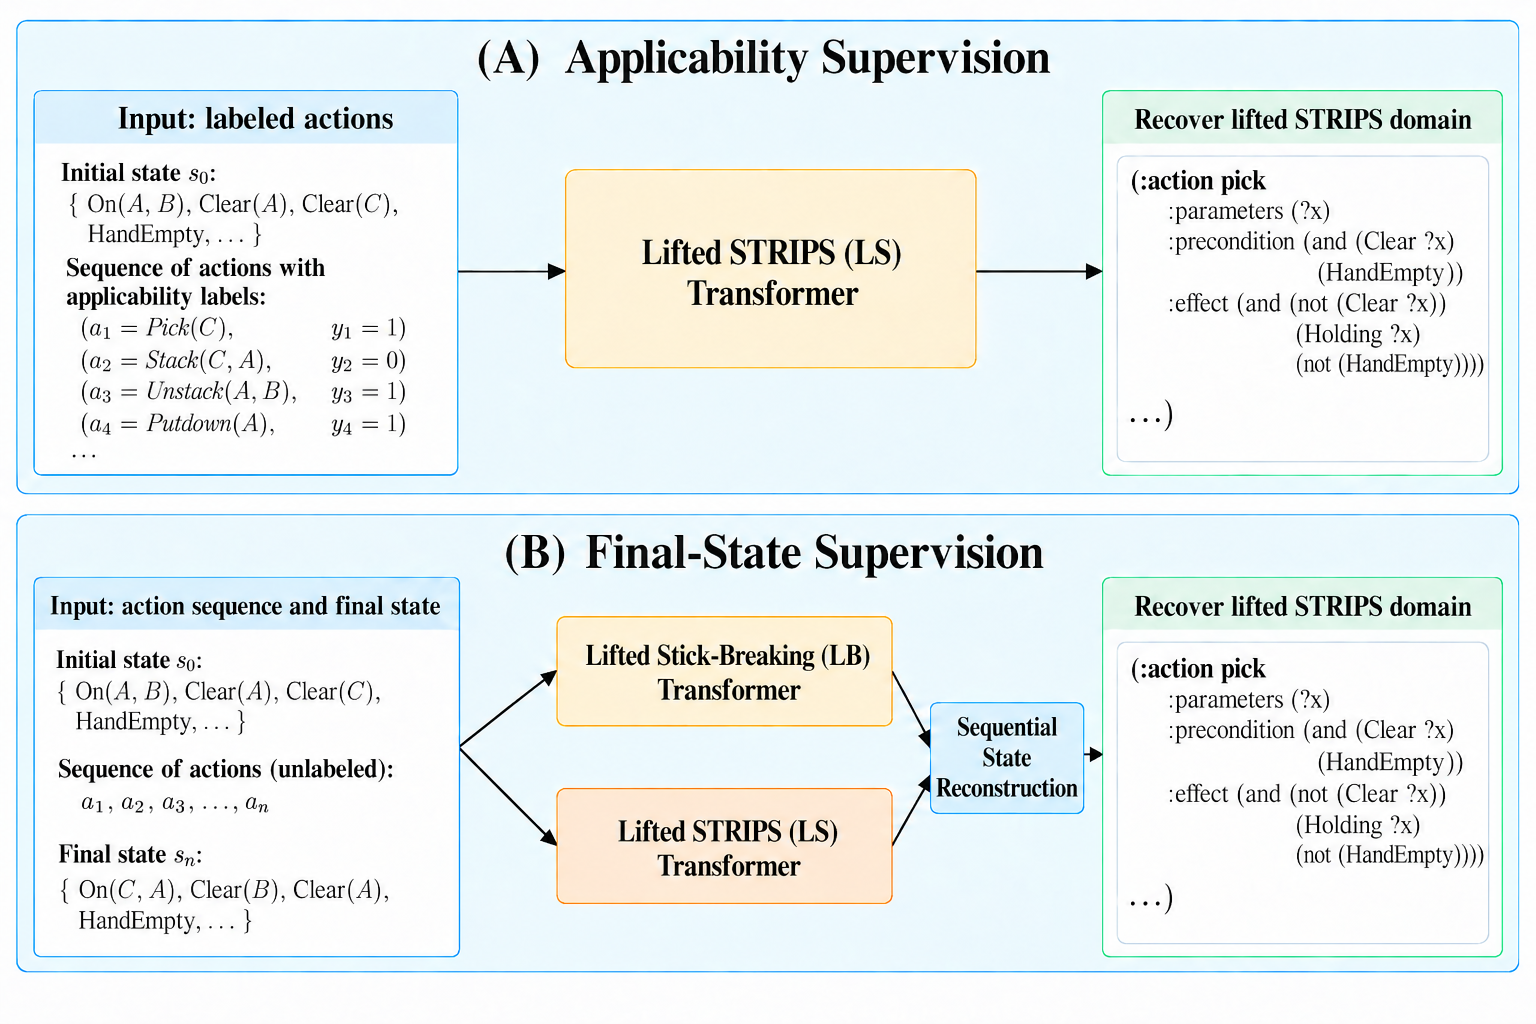
\includegraphics[width=\textwidth]{combined3_A.png}
%    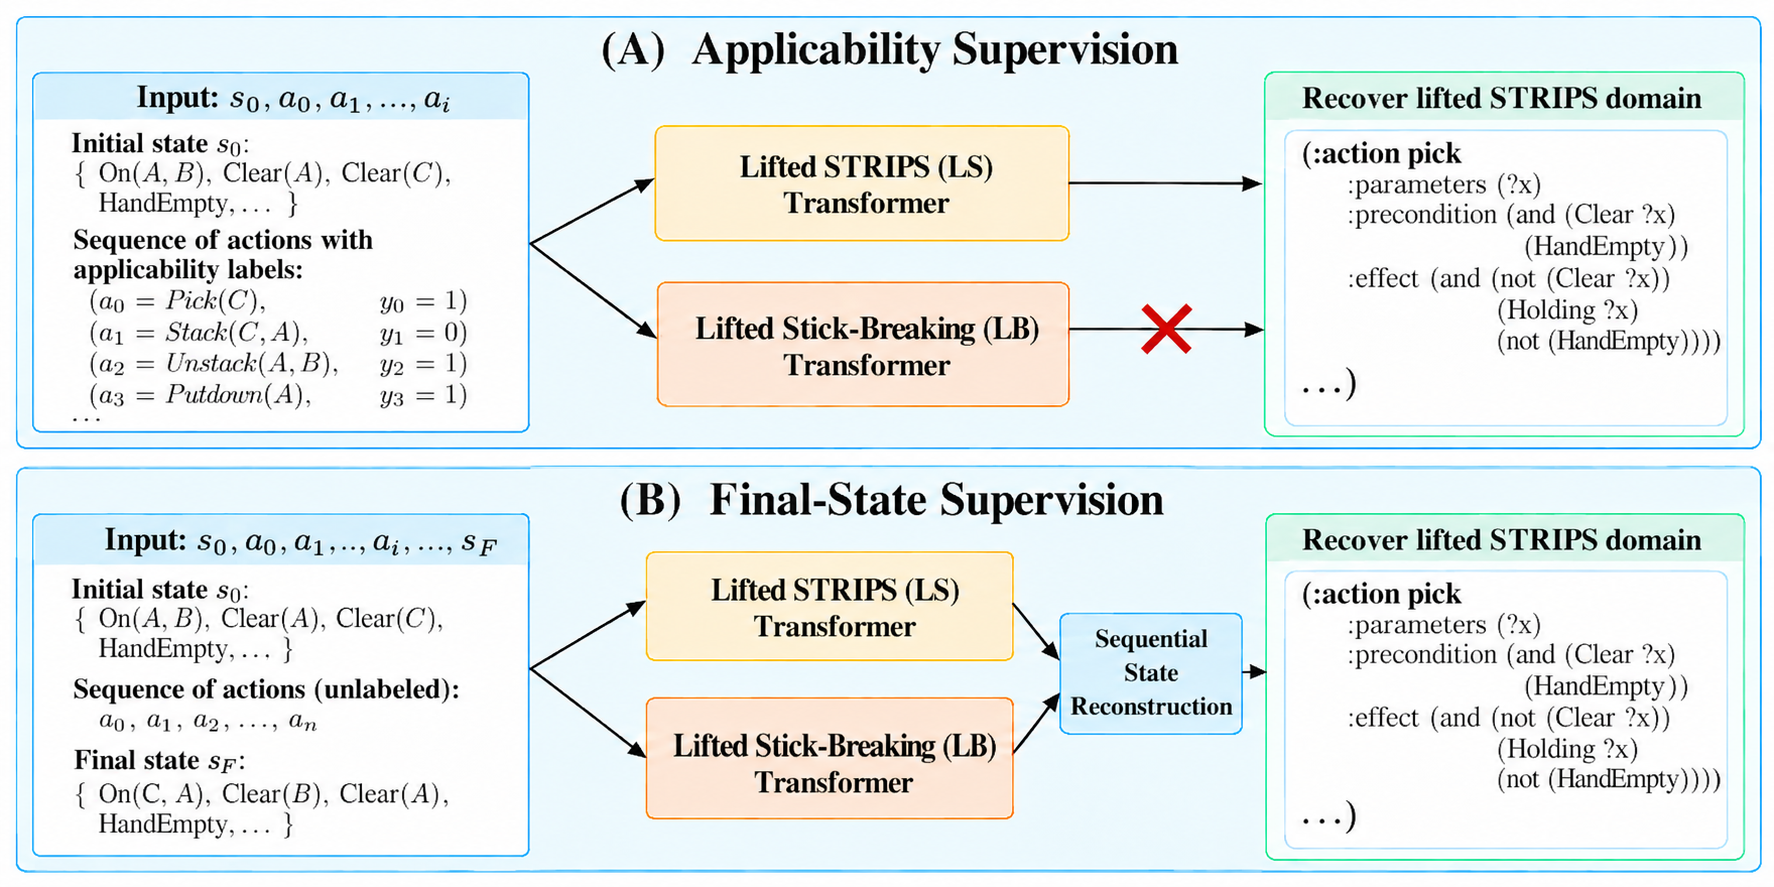
\includegraphics[width=\textwidth]{combined4_A.png}
    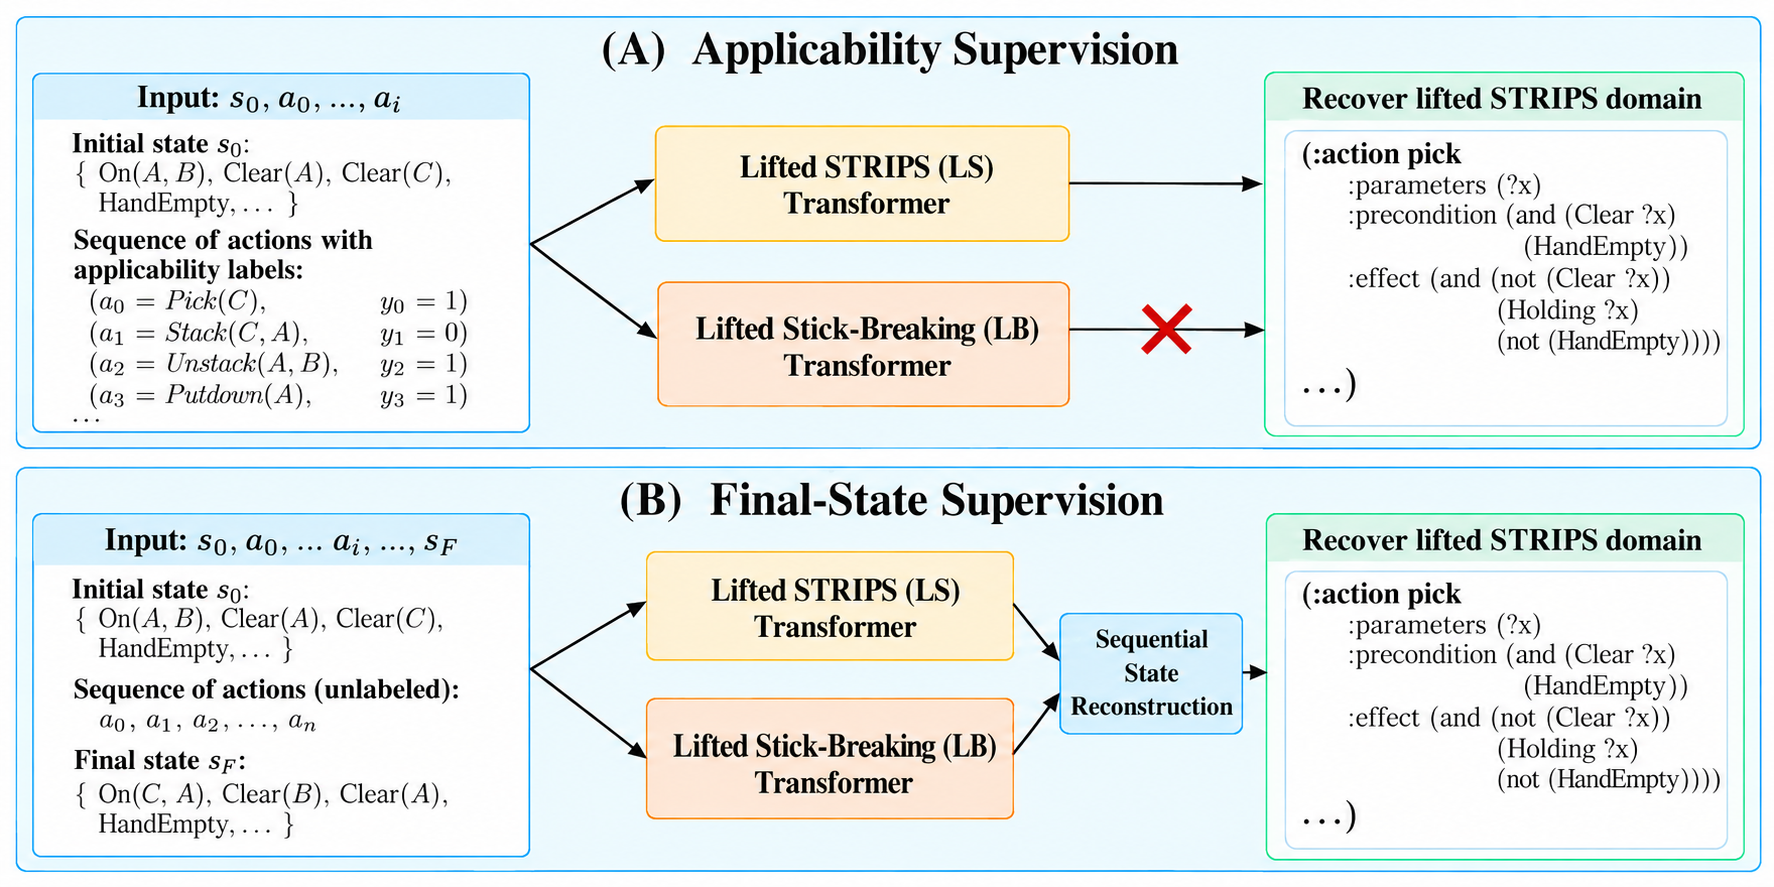
\includegraphics[width=\textwidth]{combined5_A.png}
\caption{ 
\textbf{Overview of the two architectures and supervision settings.}
We introduce the Lifted \strips (LS) Transformer, whose learned parameters are explicitly aligned with a symbolic action model, and the Lifted Stick-Breaking (LB) Transformer, an architecture closer to the standard Transformer that uses stick-breaking attention and randomized object embeddings. Both are trained from traces, each containing an initial state and an action sequence.
\textbf{(A) Applicability supervision:} actions in each trace are labeled as applicable or inapplicable, without observing any subsequent state. Only the Lifted \strips (LS) Transformer supports direct extraction of a lifted \strips model from its learned parameters.
\textbf{(B) Final-state supervision:} each trace contains the resulting final state, but no applicability labels. A lifted \strips  model is  recovered from the LS transformer as before
\hector{no state reconstruction here; fix in fig}, and from the LB transformer after inferring the intermediate states.
}
%         \caption{ \textbf{Overview of the two supervision settings.} \textbf{(A) Applicability supervision:} the model receives an initial state together with an action sequence whose actions are labeled as applicable or inapplicable. The Lifted \strips (LS) Transformer can be trained in this setting, and a symbolic action model can be extracted directly from its learned parameters. \textbf{(B) Final-state supervision:} the model receives an initial state, an applicable action sequence, and its resulting final state, but no applicability labels. In this more conventional setting, transformer variants can be trained, including the Lifted Stick-Breaking (LB) Transformer, which uses stick-breaking attention and randomized object embeddings, as well as the LS Transformer. A lifted symbolic model can then be recovered through a sequential state reconstruction procedure.        }
      \label{fig:applicability}
\end{figure*}

Our results show that both the LS and LB Transformers recover lifted world models that generalize to longer traces and to problem instances with more objects than those seen during training, whereas standard Transformer variants with softmax attention and positional encodings fail to recover the correct model. With final-state supervision, both architectures recover a \strips model through sequential state reconstruction, while with applicability supervision the LS Transformer recovers it directly, without observing any state after the initial one.

The two transformer architectures are extensions of the ones considered by \citep{nunez2026strips} for learning lifted rather than propositional models, and for dealing with different types of inputs.
The Lifted \strips transformer represents lifted \strips models in parametric form, and such  models can be extracted from the trained transformer in a direct manner.
The Lifted Stick-Breaking Attention transformer or LB-transformer, on the other hand, is a vanilla-like transformer but with a slightly different attention mechanism that replaces
softmax attention  by stick-breaking attention \citep{tan2025scaling} and which  randomizes  object embeddings in order  to  generalize across objects.
% The lifted \strips (LS) Transformer is instead symbolically aligned, with parameters that correspond directly to a lifted action model, extending the propositional architecture of~\citet{nunez2026strips} and its connection to masked hard-attention transformers~\citep{yang2024masked}.
The LB-transformer can  be trained and tested in the two learning settings where it generalizes well in length and number of objects,
but it produces a \strips model only in the second learning setting where the final state is included in the training traces.
Moreover, the model  cannot be read directly from the transformer parameters. Instead, the trained transformer is used to infer
the intermediate states between the initial and final states of the the traces, and then a simple, standard algorithm infers
the lifted action model from the full  state-action sequence thus reconstructed.  Figure~\label{fig:applicability} illustrate
the two learning settings and the inputs and outputs of the two transformers.


Our main contributions are:


\begin{itemize}
\item Two new  architectures for learning lifted \strips models:  the LS and LB transformers.
\item Two new supervised learning settings for this task:  one where action sequences (and subsequences) are labeled as applicable or not given an initial state,
and another one, where applicable action sequences from an initial state are labeled with the resulting, final states.
\item Experimental results that show generalization to longer traces with more objects, and nearly perfect model learning and planning.
\end{itemize}

In addition, following Nunez-Molina et al. (2026) we provide a B-RASP formulation of lifted \strips trace recognition, which is the basis of the LS-transformer.


\Omit{Original Intro 

A question in learning world models from sequential experience is whether models trained on finite traces recover dynamics that remain valid beyond the training data~\citep{Toshniwal_Wiseman_Livescu_Gimpel_2022,li_iclr,nanda2023linear,world-models2}. Such models should generalize as traces become longer or environments larger~\citep{vafa2025what}, while providing interpretable rules that can be inspected and applied beyond the observed traces when reasoning and planning are required.

One convenient representation for this purpose is \strips, a logic-based language in which action rules are expressed over variables rather than particular objects, allowing the same rules to apply to problem instances with different numbers of objects~\citep{russell:book,ghallab:book,geffner:book}.

Here we study whether transformer-based sequence models can learn such lifted representations from symbolic traces containing an initial state and actions instantiated with concrete (grounded) objects, but no intermediate-state observations. We evaluate whether the learned models transfer to unseen initial states and problem instances with more objects, where new objects induce actions not encountered during training, while composing correctly over substantially longer action sequences.

We take two complementary angles. The first concerns supervision, for which we consider two learning settings, building on recent work on action-model learning under limited observability~\citep{jansen2025incomplete,gosgens2026minimal}. In the \emph{applicability} setting, the final state is omitted and actions are instead labeled according to whether they can be executed. In the \emph{final-state} setting, executable action sequences are given together with their resulting final states.

The second angle concerns architectural inductive bias. We introduce two transformer-based models with different structural priors. The Lifted Stick-Breaking (LB) Transformer remains close to a standard Transformer while using stick-breaking attention~\citep{tan2025scaling} and randomized object embeddings to promote generalization across trace lengths and object identities. The lifted \strips (LS) Transformer is instead symbolically aligned, with parameters that correspond directly to a lifted action model, extending the propositional architecture of~\citet{nunez2026strips} and its connection to masked hard-attention transformers~\citep{yang2024masked}.

\begin{figure*}[!t]
    \centering    
%    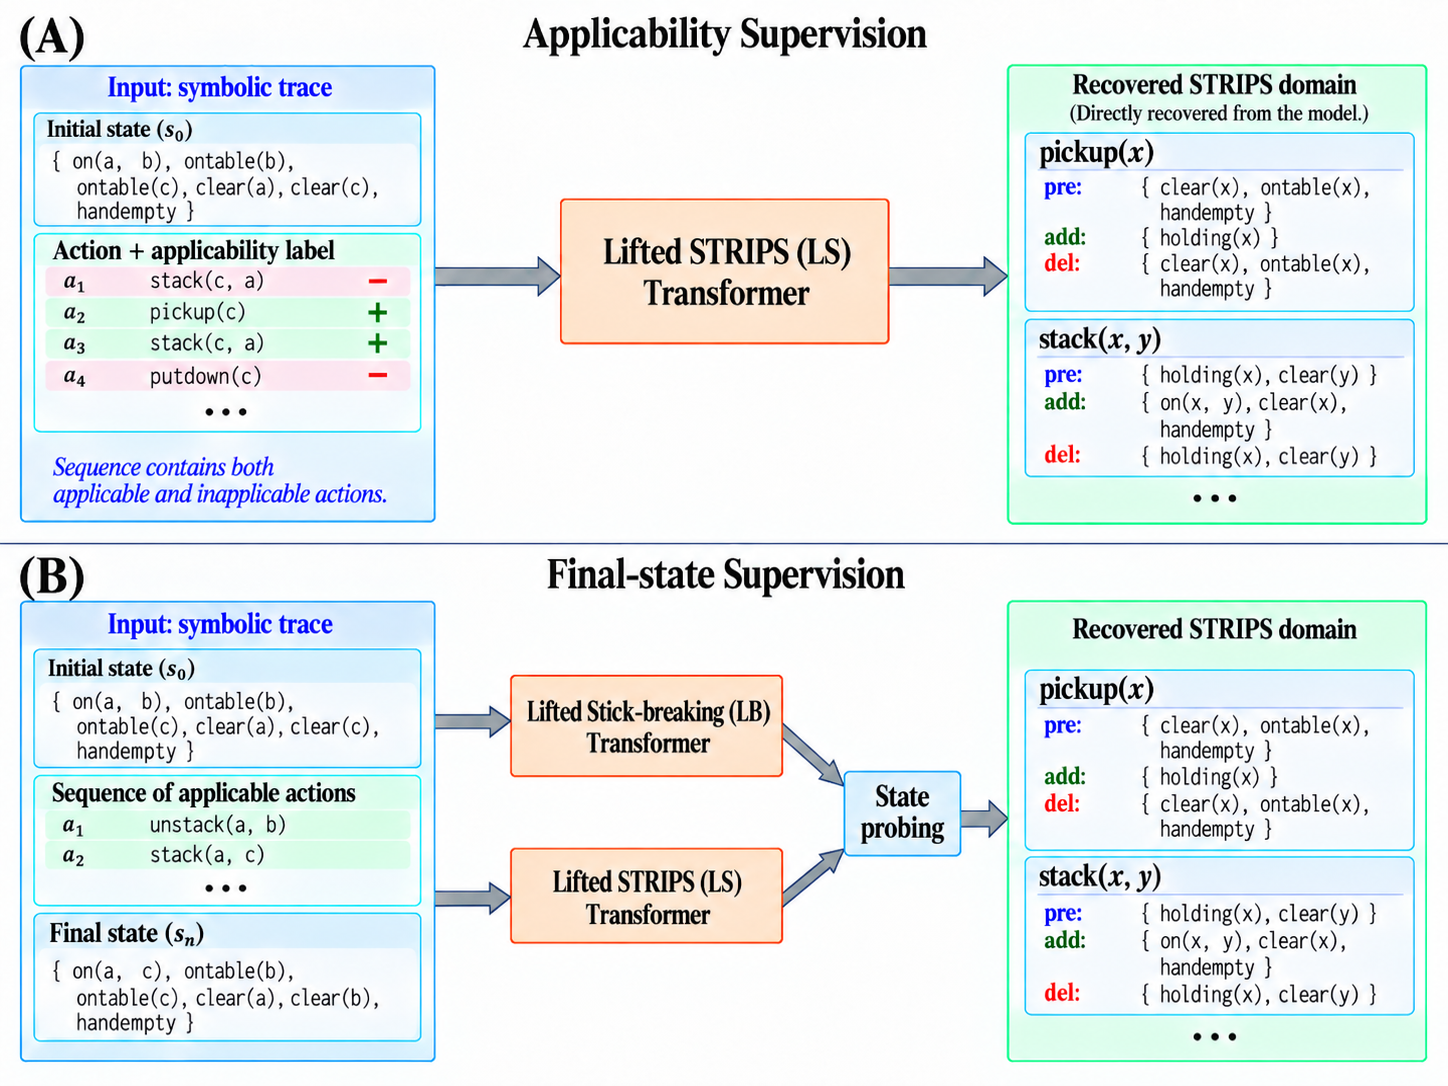
\includegraphics[width=\textwidth]{combined2_A.png}
%    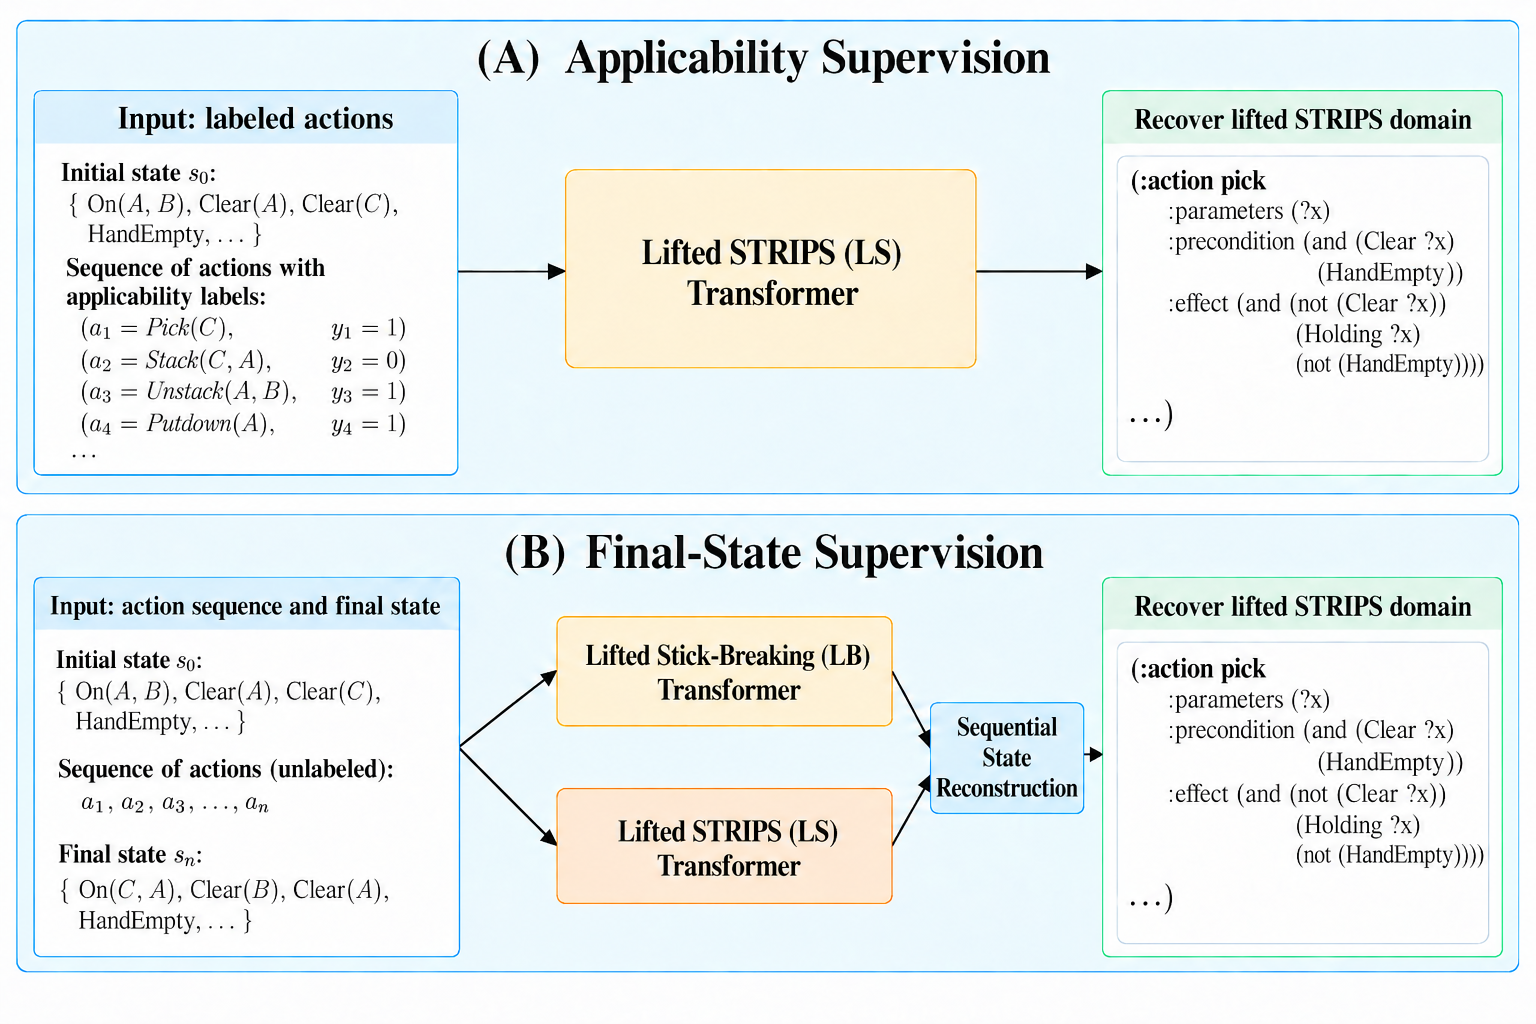
\includegraphics[width=\textwidth]{combined3_A.png}
%    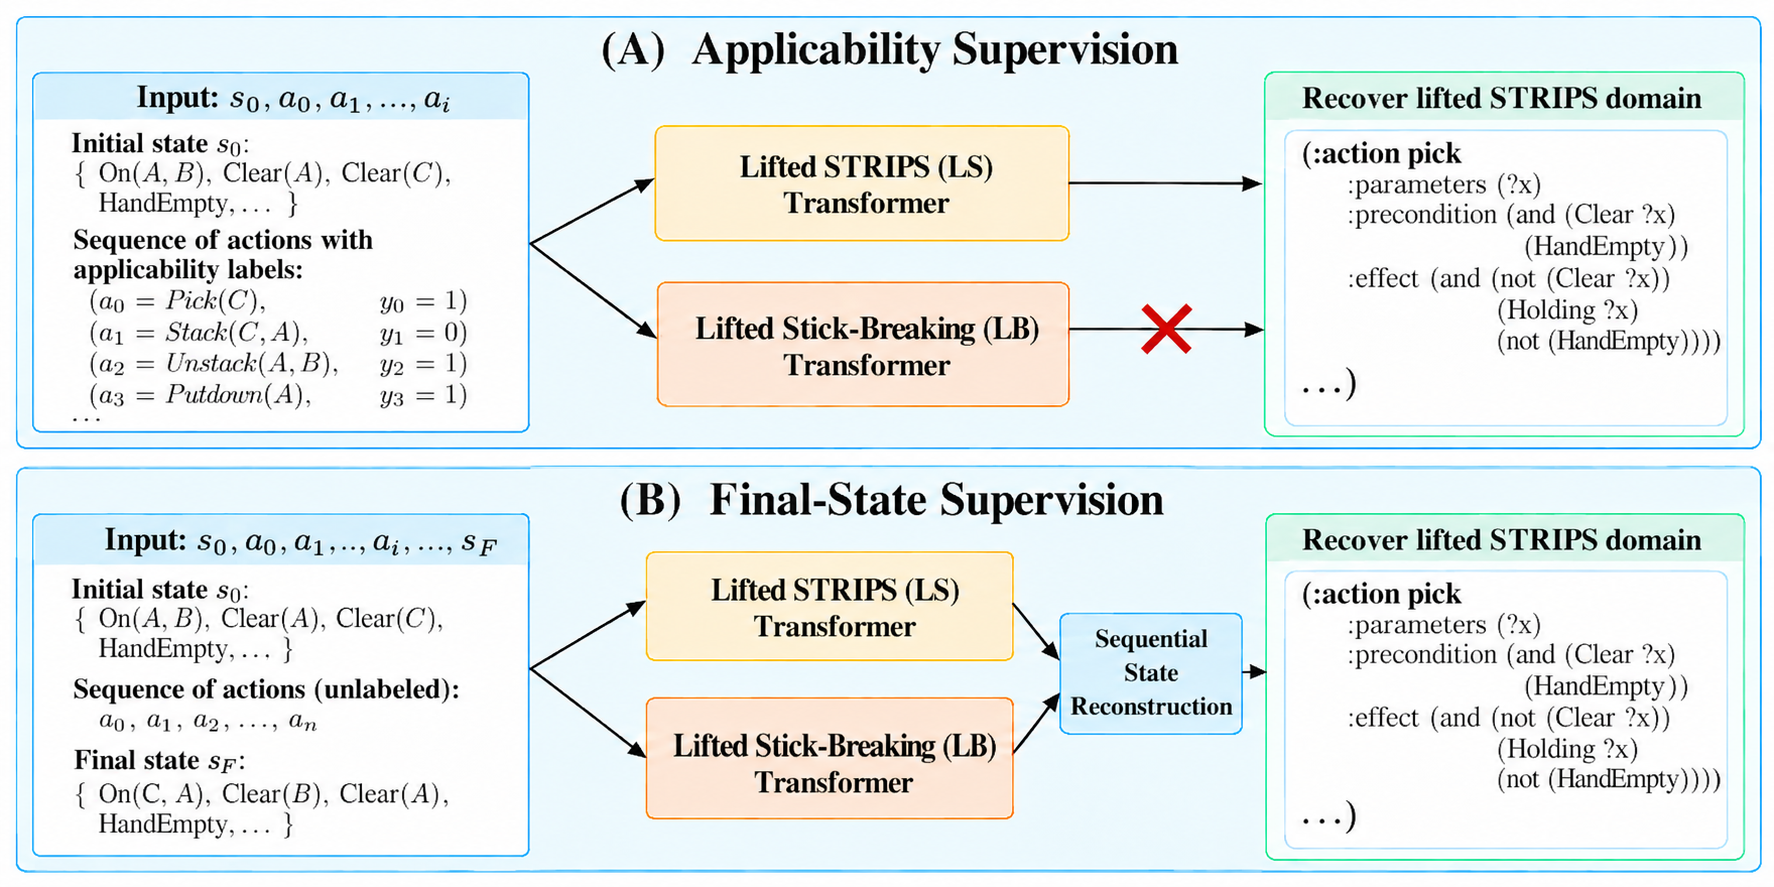
\includegraphics[width=\textwidth]{combined4_A.png}
    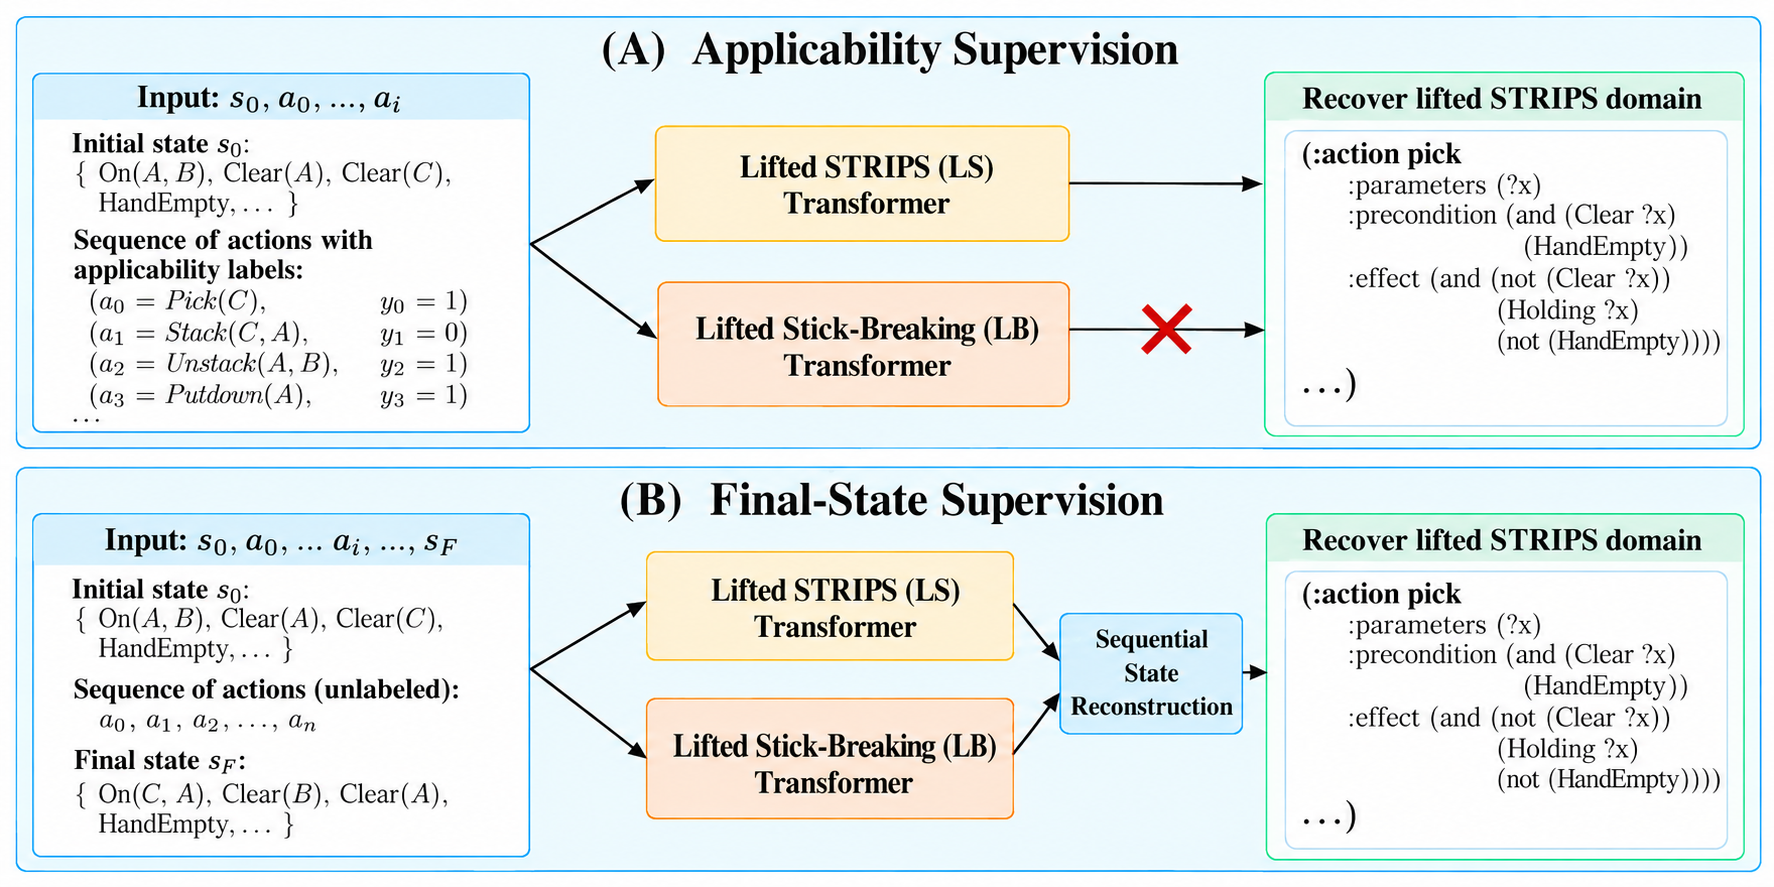
\includegraphics[width=\textwidth]{combined5_A.png}
\caption{ 
\textbf{Overview of the two architectures and supervision settings.}
We introduce the Lifted \strips (LS) Transformer, whose learned parameters are explicitly aligned with a symbolic action model, and the Lifted Stick-Breaking (LB) Transformer, an architecture closer to the standard Transformer that uses stick-breaking attention and randomized object embeddings. Both are trained from traces, each containing at least an initial state and an action sequence.
\textbf{(A) Applicability supervision:} actions in each trace are labeled as applicable or inapplicable, without observing any subsequent state. Only the Lifted \strips (LS) Transformer supports direct extraction of a symbolic action model from its learned parameters.
\textbf{(B) Final-state supervision:} each trace contains an initial state, an action sequence consisting only of applicable actions, and the resulting final state, but no applicability labels. A lifted symbolic model can be recovered from either architecture through a sequential state reconstruction procedure.
}
%         \caption{ \textbf{Overview of the two supervision settings.} \textbf{(A) Applicability supervision:} the model receives an initial state together with an action sequence whose actions are labeled as applicable or inapplicable. The Lifted \strips (LS) Transformer can be trained in this setting, and a symbolic action model can be extracted directly from its learned parameters. \textbf{(B) Final-state supervision:} the model receives an initial state, an applicable action sequence, and its resulting final state, but no applicability labels. In this more conventional setting, transformer variants can be trained, including the Lifted Stick-Breaking (LB) Transformer, which uses stick-breaking attention and randomized object embeddings, as well as the LS Transformer. A lifted symbolic model can then be recovered through a sequential state reconstruction procedure.        }
        \label{fig:applicability}
\end{figure*}
Our results show that both the LS and LB Transformers recover lifted world models that generalize to longer traces and to problem instances with more objects than those seen during training, whereas standard Transformer variants with softmax attention and positional encodings fail to recover the correct model. With final-state supervision, both architectures recover a \strips model through sequential state reconstruction, while with applicability supervision the LS Transformer recovers it directly, without observing any state after the initial one.

Our main contributions are:
\begin{itemize}
\item We introduce the Lifted \strips (LS) Transformer and the Lifted Stick-Breaking (SB) Transformer, \textbf{two transformer architectures for lifted world-model learning} with different structural biases and trade-offs.
\item We provide a \textbf{B-RASP formulation of lifted \strips trace recognition} and show that the LS Transformer provides a differentiable realization of this computation.
\item We study \textbf{two complementary forms of supervision} that trade off different sources of information. Final-state supervision learns from executable action sequences together with their resulting final states, whereas applicability supervision uses applicable and inapplicable actions without observing any subsequent state.
\item Across five planning domains, we demonstrate \textbf{generalization to substantially longer traces and problem instances with more objects than seen during training}. The LS Transformer achieves perfect generalization in the final-state setting and yields explicit lifted models that can be used for planning.
\end{itemize}
%\textbf{Carlos -- Provide main features/advantages of each transformer.}

%STRIPS Transformer. Parameters are continuous/soft approximation of lifted STRIPS models. Thus, there is one-to-one correspondence between quantized/binarized parameters and lifted STRIPS models. Also, to the best of our knowledge, it is the only Deep Learning-based method capable of learning world models without observing state transitions (\textit{risky claim, but I think it is true and an important contribution}).

%SB Transformer. Based on standard soft-attention transformer. Inspired by vector-symbolic architectures. Object tokens as non-learnable random embeddings. This forces the transformer to learn \textit{lifted equality} $x==y$, regardless of the particular objects $x,y$ represent. Therefore, it exhibits object generalization \textit{by design}.

% expand abstract ; picture of basic learning task, architecture, ...
%- Perhaps a Preview Section: concrete inputs, outputs

%In recent years, many works have considered whether transformers, and LLMs by extension, can learn world models as a result of performing next-token prediction. In this paper, we focus on world models expressed in STRIPS, a formal language based on first-order logic.

%STRIPS models possess two main advantages over neural world models. First, they are fully interpretable, since they are encoded as a set of logic rules. Second, they are lifted, meaning they generalize to tasks with any number of objects.

%We consider two alternative learning settings. In the applicability setting, each training trace encodes its initial state and a sequence of applicable and inapplicable actions, but contains no information about successor states. In the state prediction setting, traces encode their initial and final states, but do not include inapplicable actions.

%We perform experiments on five classical planning domains using both learning settings and transformers. Results show both transformers learn successfully across all domains. They achieve high training and test accuracy, generalizing to both longer traces and tasks with more objects. Additionally, they exhibit robust reasoning capabilities, as the extracted STRIPS models support planning via off-the-shelf symbolic algorithms.

}
